\subsubsubsubsection{Roadway Factory}
\begin{figure}[h]
\centering
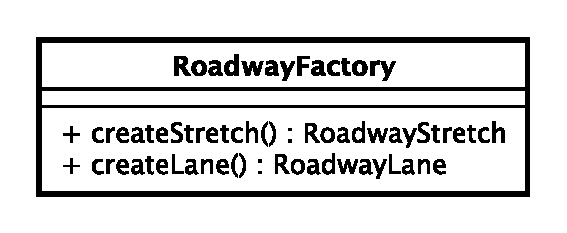
\includegraphics[scale=0.6,keepaspectratio]{images/solution/roadway_factory.eps}
\caption{App::Reactive::RoadwayFactory}
\label{fig:sd-app-roadway-factory}
\end{figure}
\FloatBarrier
\begin{itemize}
  \item \textbf{Description} \\
It represents a factory which creates roadway components.
  \item \textbf{Operation} \\
  \begin{itemize} 
    \item \texttt{+ createStretch() : RoadwayStretch} \\
Creates a new roadway stretch component.
    \item \texttt{+ createLane() : RoadwayLane} \\
Creates a new roadway lane component.
  \end{itemize}
\end{itemize}
